% Estas slides tienen que abrirse con el programa pdfpc que soporta videos embebidos
% el comando es: pdfpc -g slides.pdf
% para los videos se requiere ubuntu-restricted-extras
% para la bibliografía se requiere biber y configurar texstudio

%\documentclass[compress,handout]{beamer}
\documentclass[aspectratio=169,compress]{beamer}

% add beamer preamble
% In this preamble should go only package and settings related with beamer

% Theme customization
\setbeamertemplate{itemize item}[rectangle] % configure itemize
\setbeamertemplate{itemize subitem}[circle] % configure itemize
\setbeamertemplate{itemize subsubitem}[triangle] % configure itemize
\setbeamertemplate{navigation symbols}{} % remover simbolos de navegacion de las slides
\usefonttheme[onlymath]{serif} % simbolos matematicos en serif (Como es en latex original)
\setbeamersize{text margin left=3mm,text margin right=3mm} 

\setbeamertemplate{blocks}[rounded] % blocks corners rounded
\setbeamercolor{block body}{bg=blue!12,fg=black} % color of blocks
\setbeamertemplate{caption}{\raggedright\insertcaption\par} % elimina la palabra "Figura" del caption

\usepackage[overridenote]{pdfpc} % requires to download manually pdfpc.sty package from https://www.ctan.org/pkg/pdfpc


% HOW TO SHOW ADDITIONAL SLIDES%
\newif\ifadditional % conditional to show additional slides
%\additionaltrue   % uncomment to show additional slides
\additionalfalse % uncomment to show without additional slides

% Reference cite without footnote mark
\newrobustcmd*{\footfullcitenomark}{%
    \AtNextCite{%
        \let\thefootnote\relax
        \let\mkbibfootnote\mkbibfootnotetext}%
    \footfullcite}


% add latex preamble
% para la bibliografía se requiere biber y configurar texstudio

% Latex packages
\usepackage[utf8]{inputenc}
\usepackage[T1]{fontenc} % para copiar acentos en español del pdf y permite acentos en las notas
\usepackage[spanish]{babel}
\usepackage[per-mode = symbol]{siunitx} % para manejar las unidades
\usepackage{multimedia} % to add videos with \movie command
\usepackage{multirow}
\usepackage{graphicx}
\usepackage{xcolor}
\usepackage{amsmath} % bmatrix
\usepackage[makeroom]{cancel} % \cancel to cancel terms in math equations
\renewcommand{\CancelColor}{\color{red}} % set red color for \cancel command
\usepackage[caption=false]{subfig} % caption = false elimina la palabra "Figura" del caption
\usepackage{import} % para el comando import (se usa para pdf_tex)
\captionsetup[subfigure]{labelformat=empty} % remover el indice del caption de la subfigura
\usepackage{booktabs} % \toprule \midrule \bottomrule
\usepackage[backend=biber]{biblatex} % set biber to format references. Must configure Biber in Texstudio
\usepackage{csquotes} % to remove warning triggered by biblatex and babel
\usepackage{algpseudocode} % to write algorithm
\usepackage{tikz} % to use tikz
\usepackage[export]{adjustbox} %valign in subfloat
\usepackage{colortbl} % to paint cells in a table

% Color commands for annotations
\newcommand\TODO[1]{\textbf{\textcolor{red}{#1}}} %  TODO notes

% Graphic paths
\graphicspath{{./images/}}

% listings configuration for C code
\usepackage{listings} % code
\definecolor{commentgreen}{RGB}{2,112,10}
\definecolor{eminence}{RGB}{108,48,130}
\definecolor{weborange}{RGB}{255,165,0}
\definecolor{frenchplum}{RGB}{129,20,83}

\lstset{ % spanish characters for listings package
	inputencoding=latin1,
    columns=fullflexible,
	breaklines=true,
	tabsize=2,
	showstringspaces=false,
	basicstyle=\ttfamily,
	backgroundcolor=\color{lightgray}, % Choose background color
	literate={á}{{\'a}}1
	{ã}{{\~a}}1
	{é}{{\'e}}1
	{ó}{{\'o}}1
	{í}{{\'i}}1
	{ñ}{{\~n}}1
	{¡}{{!`}}1
	{¿}{{?`}}1
	{ú}{{\'u}}1
	{Í}{{\'I}}1
	{Ó}{{\'O}}1
    {-}{-}1
}

\lstdefinestyle{cpp}{ % spanish characters for listings package
    language=C++,
   	commentstyle=\color{commentgreen},
    keywordstyle=\color{eminence},
    stringstyle=\color{red},
    emph={int,char,double,float,unsigned,void,bool},
    emphstyle={\color{blue}}
}

\lstdefinestyle{bash}{ % spanish characters for listings package
	language=Bash
}

\lstdefinestyle{xml}{
	language=XML,
	morekeywords={encoding,xs:schema,xs:element,xs:complexType,xs:sequence,xs:attribute}
}

\lstdefinestyle{cmake}{
	language=make, % there is no cmake support in listings
}

\lstdefinestyle{python}{
    language=python,
}


%%%%% PARA QUE EN LAS TABLAS SE PUEDA PONER UN SALTO DE LINEA DENTRO DE UNA CELDA
\newcommand{\specialcell}[2][c]{%
    \begin{tiny}
        \begin{tabular}[#1]{@{}c@{}}#2\end{tabular}  
    \end{tiny}
}
%%%%%%%%%%%%%%%%%%%%%%%%%%%%%%%%%%%%%%%%%%%%%%%%%%%%%%%%%%%%%%%%%%%%%%%%

%%%%% PARA QUE LAS TABLAS TENGAN TODAS LAS COLUMNAS CENTRADAS Y DE IGUAL TAMAÑO
\usepackage{tabularx}
\renewcommand{\tabularxcolumn}[1]{>{\centering\arraybackslash}m{#1}}
%%%%%%%%%%%%%%%%%%%%%%%%%%%%%%%%%%%%%%%%%%%%%%%%%%%%%%%%%%%%%%%%%%%%%%%%



% add math preamble
\usepackage{amsmath}
\usepackage{amssymb}
\usepackage{amsopn}
\usepackage{mathtools}
\usepackage{nicematrix} % Add colors to matrix


% set matrix maximum length
\setcounter{MaxMatrixCols}{20}

% math
\renewcommand{\vec}[1]{\boldsymbol{\mathbf{#1}}}
\newcommand{\norm}[1]{\lVert#1\rVert}

% Declare arg max and arg min functionss
\DeclareMathOperator*{\argmax}{arg\,max}
\DeclareMathOperator*{\argmin}{arg\,min}

% Declare atan2 
\DeclareMathOperator{\atantwo}{atan2}

% Homogeneous decoration function
\newcommand{\homo}[1]{\dot{#1}}


% Declare projection as math function
\DeclareMathOperator{\proj}{proj}
\newcommand{\fromCoord}[2]{{#1}_\mathrm{#2}}
\newcommand{\toCoord}[2]{\prescript{\mathrm{#2}}{}{#1}}
\newcommand{\worldCoordSystem}{\mathrm{W}}
\newcommand{\bodyCoordSystem}{\mathrm{B}}
\newcommand{\cameraCoordSystem}{\mathrm{C}}
\newcommand{\origin}{\vec{o}}
\newcommand{\point}{\vec{p}}
\newcommand{\worldPoint}{\toCoord{\point}{\worldCoordSystem}}
\newcommand{\imagePoint}{\vec{u}}
\newcommand{\cameraPoint}{\toCoord{\point}{\cameraCoordSystem}}
\newcommand{\homoWorldPoint}{\toCoord{\homo{\point}}{\worldCoordSystem}}
\newcommand{\homoImagePoint}{\homo{\imagePoint}}
\newcommand{\homoCameraPoint}{\toCoord{\homo{\point}}{\cameraCoordSystem}}
\newcommand{\measurement}{\vec{z}}
\newcommand{\prediction}{\hat{\vec{z}}}
\newcommand{\seMatrix}{\vec{\xi}}
\newcommand{\transform}[2]{\toCoord{\fromCoord{\seMatrix}{#2}}{#1}}
\newcommand{\pointCoord}[1]{\toCoord{\point}{#1}}
\newcommand{\rotation}{\vec{R}}
\newcommand{\rotationCoord}[2]{\toCoord{\fromCoord{\rotation}{#2}}{#1}}
\newcommand{\translation}{\vec{t}}
\newcommand{\translationCoord}[2]{\toCoord{\fromCoord{\translation}{#2}}{#1}}
\newcommand{\intrinsicMatrix}{\vec{K}}
\newcommand{\principalPoint}{\vec{c}}
\newcommand{\reprojectionError}{u}
\newcommand{\projectionMatrix}{\vec{P}}
\newcommand{\cameraCenter}{\vec{o}}
\newcommand{\worldCameraCenter}{\toCoord{\cameraCenter}{\worldCoordSystem}}
\newcommand{\essentialMatrix}{\vec{E}}
\newcommand{\fundamentalMatrix}{\vec{F}}
\newcommand{\inverse}[1]{{#1}^{-1}}
\newcommand{\epipole}{\vec{e}}

% Localization (State Estimation)
\newcommand{\state}{x}
\newcommand{\observation}{z}
\newcommand{\controlCommand}{u}
\newcommand{\covariance}{\Sigma}
\newcommand{\motionModelNoise}{\epsilon}
\newcommand{\measurementModelNoise}{\delta}
\newcommand{\motionModelFunction}[1]{g\left( #1 \right)}
\newcommand{\observationModelFunction}[1]{h\left( #1 \right)}
\newcommand{\motionParametersCovariance}{R}
\newcommand{\observationModelCovariance}{Q}
\newcommand{\motionModelJacobian}{G}
\newcommand{\observationModelJacobian}{H}
\newcommand{\kalmanGain}{K}
\newcommand{\normalDistribution}[2]{\mathcal{N}\left( {#1}, {#2} \right)}
\newcommand{\motionModelJacobianControl}{V}
\newcommand{\motionModelCovariance}{M}
\newcommand{\stateEvolutionMatrix}{A}

% Mapping slides
\newcommand{\map}{m}
\newcommand{\mapRandomVariable}{m}

% SLAM slides
\newcommand{\informationMatrix}{\vec{\Omega}}
\newcommand{\error}{\vec{e}}
\newcommand{\observationBold}{\vec{z}}
\newcommand{\stateBold}{\vec{x}}
\newcommand{\jacobian}{\vec{J}}
\newcommand{\linearSystemb}{\vec{b}}
\newcommand{\linearSystemH}{\vec{H}}
\newcommand{\covarianceBold}{\vec{\covariance}}


% Motion Planning slides
\newcommand{\workSpace}{\mathcal{W}}
\newcommand{\obstaclesSet}{\mathcal{O}}
\newcommand{\robotInConfiguration}{\mathcal{A}}
\newcommand{\robotConfiguration}{q}
\newcommand{\configurationSpace}{\mathcal{C}}
\newcommand{\freeConfigurationSpace}{\configurationSpace_{free}}
\newcommand{\obstableConfigurationSpace}{\configurationSpace_{obs}}
\newcommand{\goalSet}{\configurationSpace_{goal}}
\newcommand{\startConfiguration}{\robotConfiguration_{I}}
\newcommand{\goalConfiguration}{\robotConfiguration_{G}}
\newcommand{\continuousPath}{\tau}
\newcommand{\motionLaw}{\gamma}
\newcommand{\robotActionSpace}{\mathcal{U}}


% Motion model
\newcommand{\position}{\vec{p}}
\newcommand{\orientation}{\vec{O}}
\newcommand{\orientationQuaternion}{\vec{q}}
\newcommand{\predictedPosition}{\hat{\vec{p}}}
\newcommand{\predictedOrientationQuaternion}{\hat{\vec{q}}}
\newcommand{\linearVelocity}{\vec{v}}
\newcommand{\angularVelocity}{\vec{\omega}}

\DeclareMathOperator{\slerpOp}{slerp}
\newcommand{\slerp}[1]{\slerpOp{\left( #1 \right)}}

% Map structure
\newcommand{\keyframesSet}{K}
\newcommand{\mapPointsSet}{P}
\newcommand{\observedMapPoints}{O}
\newcommand{\covisibilityKeyframes}{CK}
\newcommand{\localMap}{local\_map}

% Bundle Adjutment
\newcommand{\update}{\vec{\delta}}
\newcommand{\incremental}{\hat{\update}}


% Loop Closure names

% scaled operators and letters to fancy view
\newcommand{\sminus}{\scalebox{0.5}[1.0]{$-$}}
\newcommand{\splus}{\scalebox{0.6}[0.6]{$+$}}
\newcommand{\curr}{c}
\newcommand{\sind}[1]{\scalebox{0.6}[0.6]{$#1$}}
\newcommand{\ind}[1]{\scalebox{0.7}[0.7]{$#1$}}

\newcommand{\keyframe}{\vec{K}}
\newcommand{\bowVector}{\vec{v}}
\newcommand{\lcError}{\vec{\Omega}}
\newcommand{\relativeTransformation}{\seMatrix}
\DeclareMathOperator{\interpolate}{interpolate}

\newcommand{\relativeMotion}{\vec{\delta}}
\newcommand{\groundTruth}[1]{{#1}^{*}}

% definición del operador rot()
\DeclareMathOperator{\rotationOp}{rot}
\newcommand{\getRotation}[1]{\rotationOp{\left( #1 \right)}}

\DeclareMathOperator{\translationOp}{trans}
\newcommand{\getTranslation}[1]{\translationOp{\left( #1 \right)}}









% add bibliography resource
\renewcommand*{\bibfont}{\footnotesize} % change bibliograhy size
\bibliography{../../common/bibliography.bib}

\subtitle{Percepción}
\title{Robótica Móvil}
\author{Taihú Pire}
\institute{Laboratorio de Robótica}
\titlegraphic{
\includegraphics[width=0.4\textwidth]{images/cifasis_logo.pdf}}
\date{}


\begin{document}

% add title page
\frame{\titlepage}

\section{Percepción}
\begin{frame}
    \frametitle{Tipos de Robots}
    
    Sensores Propioceptivos (estado interno)
    Sensores exterioceptivos (estado externo)
    
\end{frame}


\begin{frame}
    \frametitle{Sensores}
    Resistive sensors
    bend sensors, potentiometer, resistive
    photocells, ...
    Tactile sensors
    contact switch, bumpers
    Infrared sensors
    Reflective, proximity, distance sensors
    Ultrasonic Distance Sensor
    Inertial Sensors (measure the second derivatives
    of position)
    Accelerometer, Gyroscopes,
    Orientation Sensors
    Compass, Inclinometer
    Laser range sensors
    Vision
    Global Positioning System
\end{frame}




\begin{frame}
    \frametitle{Optical encoders}
    \scriptsize
    \includegraphics[width=0.45\columnwidth]{images/encoder_principle}
    \includegraphics[width=0.46\columnwidth]{images/encoder_parts}
    \footnotesize

    \begin{block}{Principio de funcionamiento}
        Consta de una fuente de iluminación, una rejilla fija que enmascara la luz, un disco rotor con una fina rejilla óptica que gira con el eje y detectores ópticos fijos. A medida que el rotor se mueve, la cantidad de luz que incide en los detectores ópticos varía según la alineación de las rejillas fijas y móviles. En robótica, la onda sinusoidal resultante se transforma en una onda cuadrada discreta utilizando un umbral para elegir entre estados claros y oscuros. La resolución se mide en ciclos por revolución (CPR). La resolución angular mínima se puede calcular fácilmente a partir de la clasificación de CPR de un codificador. Un codificador típico en robótica móvil puede tener 2000 CPR
    \end{block}
\end{frame}

\begin{frame}
    \frametitle{Optical encoders}

    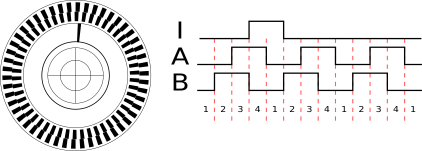
\includegraphics[width=\columnwidth]{images/encoder.pdf}
    \footnotesize

    La relación de fase observada entre los trenes de impulsos del canal A y B se utiliza para determinar la dirección de rotación. Una sola ranura en la pista interior genera un pulso de referencia (índice) por revolución.

    \begin{itemize}
        \item Proprioceptivo
        \item La resolución se mide en ciclos por revolución (CPR). Suelen tener 2000 CPR.
        \item La odometría basada en encoders acumula error rápidamente por diferencias físicas en en las ruedas, deslizamiento o giro en el aire de las ruedas.
    \end{itemize}
\end{frame}

\begin{frame}
    \frametitle{Bumper}

\end{frame}


\begin{frame}
    \frametitle{Compass}

        \includegraphics[width=0.4\columnwidth]{images/earth_magnetic_field.pdf}
        \includegraphics[width=0.4\columnwidth]{electromagnetism.jpg}

    \begin{block}{Principio de funcionamiento}
        La Tierra es un imán masivo pero débil. Los polos de este geomagnético son los polos magnéticos norte y sur de la Tierra, que se mueven constantemente y se encuentran a cierta distancia del eje de rotación del planeta.
        
        En cualquier punto del planeta, las líneas de flujo magnético pueden considerarse un vector $\vec{m}$ cuya magnitud y dirección pueden predecirse y trazarse con precisión. Describimos la dirección del vector en términos de dos ángulos: declinación e inclinación. Una proyección horizontal del vector $\vec{m}$ apunta en la dirección del norte magnético y el ángulo de declinación $D$ se mide desde el norte verdadero, en el sentido de las agujas del reloj hasta esa proyección. El ángulo de inclinación $I$ del vector se mide en un plano vertical hacia abajo desde la horizontal hasta $\vec{m}$. La longitud del vector, la intensidad del campo magnético, se mide con un magnetómetro en unidades de Tesla (T) y para la Tierra varía de $25-\SI{65}{\micro\tesla}$.
        
        El elemento clave de la mayoría de los magnetómetros modernos es un sensor de efecto Hall, un dispositivo semiconductor que produce un voltaje proporcional a la intensidad del campo magnético en una dirección normal al flujo de corriente. Normalmente, tres sensores de efecto Hall se empaquetan juntos y se disponen de modo que sus ejes sensibles sean ortogonales. Las tres salidas de dicho magnetómetro triaxial son los componentes del vector de intensidad del campo magnético de la Tierra m medido en la estructura del cuerpo \frame{B}.

    \end{block}
\end{frame}

\begin{frame}
    \frametitle{Compass}   
    \begin{figure}[!h]
        
        Las líneas de flujo magnético pueden considerarse un vector $\vec{m}$ cuya magnitud y dirección pueden predecirse y trazarse con precisión.
        
        \centering
        \subfloat[Magnetic field intensity]
        {
            \includegraphics[width=0.5\columnwidth]{images/magnetic_field_intensity.pdf}
        }
        \subfloat[Magnetic declination]
        {
            \includegraphics[width=0.5\columnwidth]{images/magnetic_declination.pdf}
        }\\
        \subfloat[Magnetic inclination]
        {
            \includegraphics[width=0.5\columnwidth]{images/magnetic_inclination.pdf}
        }
    \end{figure}

\end{frame}


\begin{frame}
    \frametitle{Compass}

    \begin{center}
        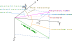
\includegraphics[width=0.5\columnwidth]{images/magnetic_field.pdf}
    \end{center}

    \begin{itemize}
        \item exteroceptivo
        \item
    \end{itemize}
\end{frame}

\begin{frame}
    \frametitle{Compass}

    \begin{center}
        \includegraphics[width=0.5\columnwidth]{pioneer_10.jpg}
    \end{center}
\end{frame}

\begin{frame}
    \frametitle{Giróscopo}

\end{frame}

\begin{frame}
    \frametitle{Acelerómetro}

\end{frame}


\begin{frame}
    \frametitle{Cámara}
    
    \note{Ver libro de Sigwart. Seccion 4.2.3.2}
    \note{material sacado de mi tesis}
    \note{https://3d.bk.tudelft.nl/courses/geo1016/slides/Lecture_03_Calibration.pdf}
    
    \begin{columns}
    	\begin{column}{0.5\textwidth}
		    \begin{figure}[!h]
			\includegraphics[width=0.6\columnwidth]{images/image_pixels.pdf}
			\end{figure}
    	\end{column}
    	\begin{column}{0.3\textwidth}
		Imagen color tiene 3 canales: R, G y B.
		\begin{equation*}
			f(x,y)=
			\begin{bmatrix}
				r(x,y) \\
				g(x,y) \\
				b(x,y)
			\end{bmatrix}
		\end{equation*}
    	\end{column}
    \end{columns}
\end{frame}

\begin{frame}
	\frametitle{Cámara}
	
%	\begin{figure}[!h]
%		\includegraphics[width=0.6\columnwidth]{images/pinhole-camera.pdf}
%	\end{figure}
\end{frame}


\begin{frame}
    \frametitle{LiDAR 2D}
    
    
    \begin{figure}[!h]
        \centering
        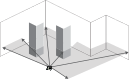
\includegraphics[width=\columnwidth]{images/lidar_example.pdf}
    \end{figure}

    \note{imagen extraida de:  https://cdn.sick.com/media/docs/3/43/443/operating_instructions_lms1104c_111031s01_2d_lidar_sensors_en_im0079443.pdf}

\end{frame}

\begin{frame}
    \frametitle{LiDAR 2D}
    
    \begin{figure}[!h]
        \centering
        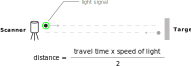
\includegraphics[width=0.6\columnwidth]{images/lidar_concept.pdf}
        
\includegraphics[width=0.35\columnwidth]{images/lidar.pdf}
    \end{figure}
    \footnotesize
    \begin{block}{Principio de funcionamiento}
     Un LiDAR (\emph{Light Detection And Ranging}) o Laser Rangefinder emite pulsos de luz mediante un diodo láser (infrarrojo). Si el rayo láser es reflejado por un objeto, el rayo reflejado es recibido por el sensor.
     
     La distancia al objeto se calcula en base al tiempo que el haz de luz pulsada requiere para ser reflejada y recibida por el sensor.
    \end{block}
    
    \begin{itemize}
        \item Extereoceptivo
        \item Activo
        \item Mide distancia y ángulo a cada punto (coordenadas polares)
        \item Unidad de medición $(\si{\meter},\si{\degree})$
    \end{itemize}

    \note{Información extraida de:  https://cdn.sick.com/media/docs/3/43/443/operating_instructions_lms1104c_111031s01_2d_lidar_sensors_en_im0079443.pdf}

\end{frame}

\begin{frame}
    \frametitle{LiDAR 2D}
    
    \begin{figure}[!h]
        \centering
        \subfloat[]
        {
            
\includegraphics[width=0.4\columnwidth]{images/lidar_range.pdf}
        }
        \subfloat[]
        {
            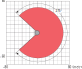
\includegraphics[width=0.55\columnwidth]{images/lidar_range2.pdf}
        }
    \end{figure}

    \note{imagenes extraida de:  https://cdn.sick.com/media/docs/3/43/443/operating_instructions_lms1104c_111031s01_2d_lidar_sensors_en_im0079443.pdf}
 
\end{frame}

\begin{frame}
    \frametitle{LiDAR 3D}

    \begin{figure}[!h]
        \centering
        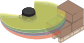
\includegraphics[width=\columnwidth]{images/lidar3d.png}
    \end{figure}

\end{frame}

\begin{frame}
    \frametitle{Cámara Time of Flight}
    \note{https://en.wikipedia.org/wiki/Time-of-flight_camera}
    
    \begin{block}{Principio de funcionamiento}
        Funciona de manera similar a un lidar con la ventaja de que toda la escena 3D se captura al mismo tiempo y que no hay partes móviles. Este dispositivo utiliza una fuente de luz infrarroja modulada para determinar la distancia de cada píxel de un sensor Photonic Mixer Device (PMD).
    \end{block}
    
    \begin{itemize}
        \item Esteroceptivo
        \item Activo
        \item La precisión suele estimarse en un $\SI{1}{\percent}$ de la distancia medida, suelen tener un frame rate de unos $\SI{160}{\hertz}$
        \item La luz del entorno mete ruido
    \end{itemize}
    
\end{frame}

\begin{frame}
    \frametitle{Ultrasónico}

\end{frame}

\begin{frame}
    \frametitle{Sensor de triangulación óptica}

    \begin{figure}[!h]
    \centering
    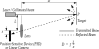
\includegraphics[width=0.7\columnwidth]{images/optical_triangulation.pdf}
    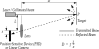
\includegraphics[width=0.25\columnwidth]{images/optical_triangulation.png}
    \end{figure}
    
\end{frame}

\begin{frame}
    \frametitle{Cámara de luz estructurada}
    \scriptsize
    \begin{center}
        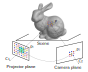
\includegraphics[width=0.3\columnwidth]{images/structured_light.pdf}
    \end{center}

    \begin{block}{Principio de funcionamiento}
        La luz estructurada (\emph{structured light}) es el proceso de proyectar un patrón conocido de píxeles (ocasionalmente rejillas o barras horizontales) en una escena. La manera en que dicho patrón se deforma cuando golpea distintas superficies permite a los sistemas de visión calcular la profundidad e información de la superficie de los objetos en la escena.
    \end{block}

    \begin{itemize}
        \item Exteroceptivo
        \item Activo
        \item No funcionan bien en entornos exteriores
        \item Corto Alcance
    \end{itemize}

\end{frame}

\begin{frame}
    \frametitle{GNSS (Global Navigation Satellite System) - Single Point Positioning (SPP)}
     \note{Página que explica como funciona un GNSS http://gutovnik.com/como_func_sist_gps.html}
     \note{video explicativo: https://youtu.be/U3eX6QKS9kY}
     \note{Slides de la estación permanente de la UNR: https://www.fceia.unr.edu.ar/gps/extension/GPSenTiempoReal.pdf}

     \begin{figure}[!h]
        \centering
        \subfloat[]
        {
            \includegraphics[width=0.2\columnwidth,valign=m]{gnss.pdf}
        }
        \hspace*{1cm}
        \subfloat[]
        {
            \movie[autostart,loop,poster]{\includegraphics[width=0.17\columnwidth,valign=m]{./images/gnss_video.jpg}}{./videos/gnss.mp4}
        }
        \subfloat[]
        {
            \includegraphics[width=0.19\columnwidth,valign=m]{gnss_satellite_orbits.pdf}
        }
    \end{figure}

    
    \begin{block}{Principio de Funcionamiento}
        Se toma la distancia a cuatro satélites (uno por cada incógnita: latitud, longitud, altitud y offset en tiempo del reloj del receptor) y se estima la pose por triangulación. La distancia a cada satélite se obtiene midiendo el tiempo que tarda en llegar la señal de radio del satélite.
    \end{block}
    
    \note{En el caso del GNSS estamos midiendo una señal de radio, que sabemos que viaja a la velocidad de la luz, alrededor de 300.000 km por segundo.}
    \note{La señal que recibe un receptor de GNSS no es solamente un Código Pseudo Aleatorio con fines de timing. También contiene un mensaje de navegación con información sobre la órbita exacta del satélite}
    \note{Otra manera de manejar los errores inducidos por la atmósfera es comparar la velocidad relativa de dos señales diferentes. Esta medición de doble frecuencia es muy sofisticada y solo es posible en receptores GNSS muy avanzados. Estos son los GNSS-RTK!}
    \note{Los receptores "normales" basados navegación por satélite, comparan una señal pseudoaleatoria que es enviada desde el satélite con una copia interna generada por la misma señal. Puesto que la señal del satélite tarda tiempo en alcanzar al receptor, las dos señales no se alinean correctamente, la copia del satélite se retrasa en referencia a la copia local. Al retrasar progresivamente la copia local, las dos señales se alinearán correctamente en algún momento. Este retraso es el tiempo necesario para que la señal alcance al receptor, y del resultado de esto puede ser calculada la distancia al satélite. La precisión de la medición resultante es generalmente una función de la capacidad  electrónica del receptor para comparar exactamente las dos señales.}
    
    \begin{itemize}
        \item Fuentes de ruido (Retrasos ionosféricos y atmosféricos, Efecto Multitrayectoria, Dilución de la Precisión, errores del reloj del satélite, imprecisión de órbita de los satélites)
        \item Error de posicionamiento métrico ($\sim\SI{2}{\meter}$)
    \end{itemize}
    
    \note{La Dilución de la Precisión (DOP) es una medida de la fortaleza de la geometría de los satélites y está relacionada con la distancia entre estos y su posición en el cielo. El DOP puede incrementar el efecto del error en la medición de distancia a los satélites.\\
    Un ejemplo de Dilución de la Precisión, si los satélites están en una misma línea (colineales) uno arriba del otro, queda como mal condicionado.}

\end{frame}

\begin{frame}
    \frametitle{Sistema GNSS-RTK (Real-Time Kinematics)}
    \footnotesize

    \begin{center}
        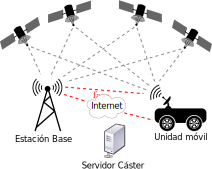
\includegraphics[width=0.3\columnwidth]{gnss_rtk_system.pdf}    
    \end{center}
    
    \only<1>{
        \begin{block}{Principio de Funcionamiento}
            \begin{itemize}
                \item Se requieren al menos dos receptores GNSS (estación base y unidad móvil). 
                \item La estación base retransmite la fase de la onda portadora de la señal enviada por el satélite \note{no tiene en cuenta los datos enviados por el satélite}
                \item La unidad móvil compara su medición de fase de la señal con la fase recibida de la estación base (\emph{Resolución de Ambig{\"u}edad})
            \end{itemize}
        \end{block}
        
        \note{ RESOLUCIÓN DE AMBIGUEDAD\\
        La sincronización entre la portadora de la señal recibida y la réplica generada en recepción permite obtener una medida de la fase de la portadora. Esta medida de fase puede ser utilizada también para estimar la distancia satélite-receptor. Sin embargo, para ello, es necesario conocer el número entero de ciclos de portadora transcurridos desde que la señal deja el satélite hasta que llega al receptor.\\
        Para realizar la sincronización entre la portadora de la señal y la réplica es necesario tener en cuenta el efecto doppler que se produce debido al movimiento relativo satélite receptor. Por ello, la frecuencia de la réplica ha de ser igual a la frecuencia de la señal transmitida con su desplazamiento doppler corregido. La sincronización se realiza mediante circuitos de enganche en fase (Phase Lock Loop, PLL) o en frecuencia (Frecuency Lock Loop, FLL). Los circuitos PLL o FLL permiten obtener medidas de fase con precisiones del orden de 0.01 ciclos de portadora.\\
        Una vez que el receptor se sincroniza con la portadora y con el código, es decir, se produce el enganche con la señal del satélite, el receptor puede medir la fase de la portadora recibida. Esta medida se obtiene de forma parecida a como se obtiene la medida de pseudodistancia, pues será el desfase que es necesario realizar a la réplica de la portadora para que se sincronice con la portadora recibida. La medida de fase se suele expresar en ciclos de portadora. Por tanto, tal como se ha descrito hasta ahora, la medida de fase será un valor decimal, no entero, indicando la fracción de ciclo de portadora transcurrido en el momento de la recepción de la señal. La distancia entre el satélite y el receptor se puede expresar en número de longitudes de onda y será igual al número entero de ciclos de portadora n transcurridos en el origen desde que la señal salió del satélite hasta que llegó al receptor, más la fracción de ciclo medida (la medida de fase). Por tanto, la medida de fase sirve como estimación de la distancia satélite-receptor pero tiene el problema de que el número entero n es desconocido. A dicho número se le denomina ambigüedad entera de ciclos de portadora. Mientras el receptor permanezca enganchado con la señal el número entero n desconocido permanecerá constante, pues el receptor registra la variación del número entero de ciclos en las propias medidas de fase. La figura 1.7 ilustra esta circunstancia. En el instante t 0 se produce el enganche, obteniéndose la medida phi 0 y siendo desconocido el número de ciclos n. A partir de entonces, el receptor registra la variación de ciclos que se van produciendo y en los instantes sucesivos las medidas de fase phi i estarán formadas por una parte fraccional y una parte entera: la diferencia entre el número de ciclos transcurridos y el número n de la medida inicial. Por tanto, el único valor desconocido es el número entero de ciclos n inicial.}
   }
    \only<2>{ 
        \begin{itemize}
            \item Error de posicionamiento submétrico ($\sim\SI{0.05}{\meter}$).
            \item Alcance de \SI{10}{\km}
            \item GNSS-RTK es una evolución de DGNSS (Differential-GNSS). GNSS-RTK utiliza un nuevo protocolo de comunicación (RTCM3) y un mejor algoritmo de corrección.
            \item NTRIP (\emph{Networked Transport of RTCM via Internet Protocol}) correcciones por internet desde una estación permanente
        \end{itemize}
        \note{DGNSS vs GNSS-RTK: https://youtu.be/SOYDTxbX4mM?si=NmRR0_DU11HEORfo}
    }
\end{frame}

\begin{frame}
    \frametitle{Estación Permamente GPS}
    \begin{center}
        \includegraphics[width=0.3\columnwidth]{gnss_ppk_system.pdf}
    \end{center}

    \href{https://www.fceia.unr.edu.ar/gps/}{https://www.fceia.unr.edu.ar/gps/}

    RINEX (\emph{Receiver Independent Exchange Format})  permite posprocesar los datos recibidos para producir un resultado más preciso, generalmente con otros datos desconocidos para el receptor original, como mejores modelos de las condiciones atmosféricas en el momento de la medición.
    RINEX es el formato estándar que permite la gestión y disposición de las medidas generadas por un receptor, así como su tratamiento off-line por multitud de aplicaciones, sea cual sea el fabricante tanto del receptor como de la aplicación informática.

\end{frame}


\begin{frame}
    \frametitle{Sistema GNSS-PPK (Post Processed Kinematic)}
    \begin{center}
        \includegraphics[width=0.3\columnwidth]{gnss_ppk_system.pdf}
    \end{center}

    El PPK (Post Processed Kinematic), a diferencia del RTK, realiza un proceso de datos a posteriori (offline).
    En la imagen vemos que, tanto la base como el drone, reciben lecturas de las diferentes constelaciones de satélites. Pero, a diferencia del RTK, no hay un enlace de datos constante entre el drone y la base, ya que ambos registran en una memoria esa información que después del vuelo deberemos descargar, normalmente en archivos con formato RINEX, para postprocesar y obtener nuestra solución.
    
\end{frame}

\begin{frame}
    \frametitle{Sistema GNSS-PPP (Precise Point Positioning)}
    \begin{center}
        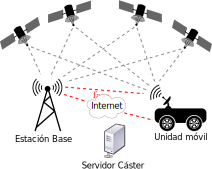
\includegraphics[width=0.3\columnwidth]{gnss_rtk_system.pdf}
    \end{center}

\end{frame}

\begin{frame}
    \frametitle{NTRIP}
    \begin{center}
        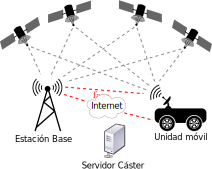
\includegraphics[width=0.3\columnwidth]{gnss_rtk_system.pdf}
    \end{center}

\end{frame}

\begin{frame}[fragile]
	\frametitle{Cámara basada en eventos}
	
	\begin{center}
		\movie[autostart,loop,poster]{\includegraphics[width=0.9\columnwidth]{images/event_camera.png}}{videos/event_camera.mp4}
	\end{center}
	
\end{frame}

\section{Bibliografía}
\section{Bibliografía}
\begin{frame}
    \frametitle{Bibliografía}
    \nocite{siegwart2011introduction}
    \nocite{corke2017robotics}
    \nocite{hartley2003multiple}
    \nocite{misra2006global}

    \printbibliography

\end{frame}

\end{document}
